
\section{Diagramma a rimbalzi}
    Si consideri il seguente circuito
    \begin{figure}[H]
        \centering
        \begin{circuitikz}
            \draw (0, 2.5) to[R, R=$Z_g$] (2, 2.5);
            \draw (2, 2.5) to[short, o-o] (7.5, 2.5);
            \draw (0, 0)   to[V, V=$V_g$] (0, 2.5);
            \draw (0, 0) to[short] (2, 0);
            \draw (2, 0) to[short, o-o] (7.5, 0);
            \draw (7.5, 0) to[R, R=$Z_L$] (7.5, 2.5);

            \draw[-latex] (1, -0.6) -- (8.5, -0.6) node[right] {$z$};
            \draw (2, -0.5) -- (2, -0.7) node[below] {$A = -l$};
            \draw (7.5, -0.5) -- (7.5, -0.7) node[below] {$B = 0$};
        \end{circuitikz}
    \end{figure}


    Si ha che
    \[
        V_A = V_g \frac{Z_A}{Z_A + Z_g}
    \]
    \[
        V_0^+ = \frac{V_A}{e^{-j k z_A} (1 + \Gamma_A)}
    \]
    \[
        V_B = V_0^+ e^{-j k z_B} (1 + \Gamma_B)
    \]

    Mettendo tutto insieme, la tensione in $z = 0$ è data da
    \[
        V_B = V_g \frac{Z_A}{Z_A + Z_g} \frac{1 + \Gamma_B}{1 + \Gamma_A} e^{-j k (z_B - z_A)} \implies v_B(t) = \mathcal{F}^{-1}\{V_B(\omega)\} 
    \]

    Qualora $Z_g$ e $Z_L$ fossero non reattivi, la linea ideale, e la forma di tensione posta dal generatore un gradino unitario o una porta, 
    sarebbe possibile trovare la soluzione nel dominio del tempo $v_B$ senza passare per l'antitrasformata di Fourier, attraverso i \textit{diagrammi di rimbalzi}.
    Prima di tutto, è necessario definire il coefficiente di riflessione del generatore $\Gamma_g$.
    Si consideri la tensione in $z=0$
    \[
        V(0) = V_g - Z_g I(0)
    \]
    Da quest'espressione si evince che la tensione in $z=0$ è data da un contributo del generatore ($V_g$) sommato ad un contributo determinato dalla linea ($-Z_g I(0)$).
    Per determinare il rapporto fra l'onda riflessa e l'onda incidente all'ingresso della linea, usiamo la sovrapposizione degli effetti e poniamo $V_g = 0$
    \[
        \begin{cases}
            V_0 = - Z_g I_0 \\ 
            V_0 = V^+_0 + V^-_0 \\ 
            I_0 = Y_\infty (V^+_0 - V^-_0) \\ 
        \end{cases}
        \implies
        V^+_0 + V^-_0 = -Z_g Y_\infty (V^+_0 - V^-_0) \implies
        \Gamma_g = \frac{V^+_0}{V^-_0} = \frac{Z_g - Z_\infty}{Z_g + Z_\infty}
    \]

    Il diagramma a rimbalzi di questo circuito, dove $\tau = l/v_f$ è il tempo di propagazione da $A$ a $B$ diventa
    \begin{figure}[H]
        \centering
        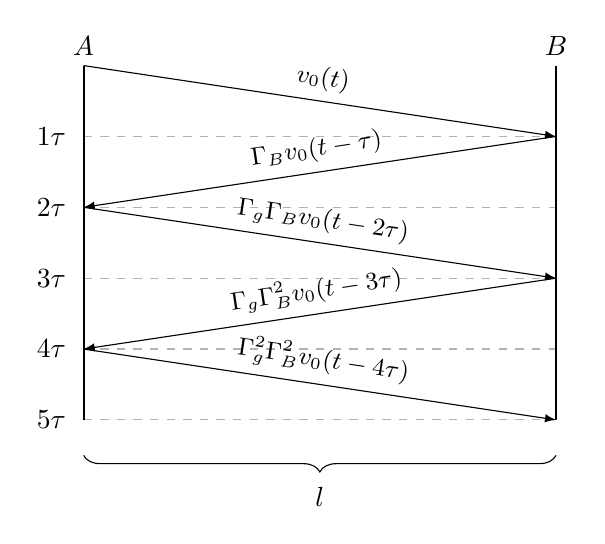
\begin{tikzpicture}[y=0.9cm]
            % Grid lines at multiples of tau
            \foreach \k in {1,...,5} {
                \draw[black!30, dashed] (0, -\k) -- (6, -\k);
                \node[left] at (-0.1, -\k) {$\k\tau$};
            }

            % Line ends: A at z = -l (left), B at z = 0 (right)
            \draw[thick] (0, 0) -- (0, -5);
            \draw[thick] (6, 0) -- (6, -5);
            \node[above] at (0, 0) {$A$};
            \node[above] at (6, 0) {$B$};

            % Forward (A to B) and backward (B to A) waves
            \draw[-latex] (0, 0) -- (6, -1) node[midway, above, sloped] {\small $v_0(t)$};
            \draw[-latex] (6, -1) -- (0, -2) node[midway, above, sloped] {\small $\Gamma_B v_0(t - \tau)$};
            \draw[-latex] (0, -2) -- (6, -3) node[midway, above, sloped] {\small $\Gamma_g\Gamma_B v_0(t - 2\tau)$};
            \draw[-latex] (6, -3) -- (0, -4) node[midway, above, sloped] {\small $\Gamma_g\Gamma_B^2 v_0(t - 3\tau)$};
            \draw[-latex] (0, -4) -- (6, -5) node[midway, above, sloped] {\small $\Gamma_g^2\Gamma_B^2 v_0(t - 4\tau)$};

            \draw[decorate, decoration={brace, mirror, amplitude=6pt}] (0, -5.5) -- (6, -5.5) node[midway, below=8pt] {$l$};
        \end{tikzpicture}
    \end{figure}

    Di conseguenza, $v_A$ e $v_B$ diventano rispettivamente
    \[
        v_A = v_0(t) + (1 + \Gamma_g) \sum_{n = 0}^{\infty} \Gamma_g^{n} \Gamma_B^{n + 1} \: v_0(t - 2(n + 1) \tau)
    \]
    \[
        v_B = (1 + \Gamma_B) \sum_{n = 0}^{\infty} \Gamma_g^{n} \: \Gamma_B^{n} \: v_0(t - (2n + 1) \tau)
    \]

    \begin{definition}[Impulso iniziale]
        Si definisce impulso iniziale la tensione all'ingresso della linea per $0 < t < 2 \tau$ qualora l'ingresso abbia forma $v_g = u(t) e(t)$.
        Tale è data dalla seguente espressione
        \[
            v_0(t) = \frac{Z_\infty}{Z_\infty + Z_g} v_g(t)
        \]
    \end{definition}


\section{Interpretazione nel dominio della frequenza}
    Tornando alla soluzione per la tensione in $B$ nel dominio della frequenza, sotto l'ipotesi di linea ideale $k = \omega \sqrt{LC}$, si ha che
    \[
        V_B = V_g \frac{Z_A}{Z_A + Z_g} \frac{1 + \Gamma_B}{1 + \Gamma_A} e^{-j k l}
    \]
    \[
        Z_g = Z_\infty \frac{1 + \Gamma_g}{1 - \Gamma_g}
    \]
    \[
        Z_A = Z_\infty \frac{1 + \Gamma_A}{1 - \Gamma_A}
    \]

    Sostituendo le impedenze $Z_A$ e $Z_g$ nella soluzione, si ottiene
    \[
        V_B = V_g \frac{1 + \Gamma_B}{(1 + \Gamma_A) + \frac{(1 + \Gamma_g)(1 - \Gamma_A)}{1 - \Gamma_g}} e^{-j k l} = 
        V_g \frac{(1 + \Gamma_B) (1 - \Gamma_g)}{2(1 - \Gamma_A \Gamma_g)} e^{-j k l} =
        V_g \frac{(1 + \Gamma_B) (1 - \Gamma_g)}{2} \frac{e^{-j k l}}{1 - \Gamma_A \Gamma_g} 
    \]

    Ricordando che $\Gamma_A = \Gamma_B e^{-2 j k l}$ e che $kl = \omega \tau$, si conclude con
    \[
        V_B = V_g \frac{(1 + \Gamma_B) (1 - \Gamma_g)}{2} e^{-j \omega \tau} \frac{1}{1 - \Gamma_g \Gamma_B e^{-2 j \omega \tau}} 
    \]

    Adesso, posta la condizione $|\Gamma_g \Gamma_B e^{-2 j \omega \tau}| = |\Gamma_g \Gamma_B| < 1$, è possibile effettuare la seguente espansione in serie
    \[
        \frac{1}{1 - \Gamma_g \Gamma_B e^{-2 j \omega \tau}} = \sum_{n = 0}^{\infty} (\Gamma_g \Gamma_B e^{-2 j \omega \tau})^n
    \]

    Ottendendo (sotto ipotesi di $Z_g$ e $Z_L$ \textbf{non} reattivi)
    \[
        V_B = V_g \frac{(1 + \Gamma_B) (1 - \Gamma_g)}{2} \sum_{n = 0}^{\infty} (\Gamma_g \Gamma_B)^n e^{-(2 n + 1) j \omega \tau}
    \]
    \begin{center}
        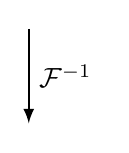
\begin{tikzpicture}
            \draw[-latex, thick] (0, 0) -- (0, -1.2) node[midway, right] {$\mathcal{F}^{-1}$};
        \end{tikzpicture}
    \end{center}
    \[
        v_B = \frac{(1 + \Gamma_B) (1 - \Gamma_g)}{2} \sum_{n = 0}^{\infty} (\Gamma_g \Gamma_B)^n v_g(t - (2n + 1) \tau)
    \]
